\pagestyle{empty} % Limpa o cabeçalho e o rodapé
\onehalfspacing % Espaçamento entre-linhas de 1,5
% \hyphenpenalty=10000 % To prevent hyphenation
\pretolerance=10000 % To avoif overful lines
%\selectlanguage{english}
\selectlanguage{brazilian}
\setcounter{ex}{0} % counter for exercises
%\pagenumbering{arabic} % Uncomment this line if you want renumber pages for each chapter
\renewcommand{\chaptername}{Tutorial}
\chapter{Suporte}\label{tut14}
\rhead{\tiny Instituto de Biociências --USP: BIZ0433 - Inferência Filogenética: Filosofia, Método e Aplicações}
\cfoot{\tiny \cc \ccby \ccsa \href{http://creativecommons.org/licenses/by-sa/4.0/}{Creative Commons Attribution-ShareAlike 4.0 International License}}
\vspace{5pt}
{\large \sc BIZ0433 - Inferência Filogenética: Filosofia, Método e Aplicações.}\par
{\sc Por Denis Jacob Machado \& Fernando P. L. Marques}\par
\vspace{10pt}
\par
\minitoc % for table of contents within the chapter
\newpage
\section*{}\addcontentsline{toc}{section}{Objetivo}
\onehalfspacing
\vspace*{5pt}
\begin{center}
\emph{\begin{large}Objetivo\end{large}}\label{tut14:Objetivo}
\vspace{2pt}
\end{center}

\begin{refsection}
\renewcommand*{\finalnamedelim}{\addspace\&\space} % Usar '&' ao invés de 'e'.

%% TEXTO DO RESUMO
O objetivo deste tutorial é apresentar conceitos teóricos e práticos do cálculo de índices de suporte em inferência filogenética. A parte conceitual é brevemente apresentada aqui e o leitor deve consultar \textcite{GrantKluge2008b}, e referências ali citadas, para uma discussão mais aprofundada sobre os aspectos epistemológicos associados à cada métrica. O tutorial inicia-se com uma apresentação geral sobre o conceito de suporte. A seguir são apresentados 3 métricas, duas das quais são comumente utilizados em análises filogenéticas. O primeiro deles é o Bootstrap, o segundo os valores de Goodman--Bremer e, finalmente, a Verossimilhança diferencial. Os arquivos associados a este tutorial estão disponíveis em \url{http://lhe.ib.usp.br/cladistica}. Você pode baixá-los diretamente com o seguinte comando:

\begin{center}
\small \texttt{wget http://lhe.ib.usp.br/downloads/tutorial\_14.zip}\\
\end{center}



\newpage
\pagestyle{fancy} % Inclui o cabeçalho definido no meta.tex
%\pagenumbering{arabic} % Números das páginas em arábicos
%% color base pairs
\newcommand{\A}{\textcolor{green}{\textbf{A}}}
\newcommand{\C}{\textcolor{blue}{\textbf{C}}}
\newcommand{\G}{\textcolor{gray}{\textbf{G}}}
\newcommand{\T}{\textcolor{red}{\textbf{T}}}
\newcommand{\gap}{\textcolor{black}{\textbf{-}}}


%%%%%%%%%%%%%%%%%%%%%%%%%%%% HERE TEXT STARTS %%%%%%%%%%%%%%%%%%%%%%%%%%%%



\begin{quote}
\scriptsize\textit{``It is sometimes observed that the measure of support does not have any 'meaning', by which is usually meant any 'probability interpretation'. It is indeed true that a statement of support, though derived from probabilities, does not make any assertion about the probability of a hypothesis being correct. And for a good reason: the method of support has been developed by people who explicitly deny that any such statement is generally meaningful in the context of a statistical hypothesis.''} \parencite[][:33]{Edwards_1992}
\end{quote}

\section{Introdução}\label{tut14:intro}

Como sugere \textcite[][]{GrantKluge2008b}, a avaliação de suporte de clados é um componente importante de análises filogenéticas, mesmo que pouca atenção tenha sido dada às bases conceituais dos métodos geralmente empregados para medi-lo. Adicionalmente, o próprio conceito de ``suporte'' difere entre cientistas, em geral, e filogeneticistas em particular. 

Em estudos filogenéticos, há uma série de métricas utilizadas para inferir índices de suporte de clados. Dentro destes índices, há aqueles considerados métricas de suporte indireto, dentro dos quais encontramos Boostrap e Jackknife -- entre outros, e métricas de suporte direto, tais como Goodman-Bremer e Verossimilhança diferencial -- entre outros. Este tutorial irá apenas abordar a implementação de algumas destas métricas. Para uma revisão mais adequada sobre o assunto é recomendável a leitura de \textcite{Siddall_2001}, \textcite{Egan_2006}, \textcite{GrantKluge2008b} e \textcite{Wheeler_2012}; e referências citadas por esses autores. 

Existem definições explícitas sobre suporte na literatura. No entanto, filogeneticistas parecem ignorá-las. Em seu livro clássico sobre Verossimilhança, \textcite{Edwards_1992} considera que índices de suporte devem aferir o mérito relativo de hipóteses rivais diante dos dados observados. Para este autor, a noção de suporte pode ser concebida por uma interpretação operacional perfeitamente simples da diferença entre as verossimilhanças entre duas hipóteses com relação aos dados. Neste contexto, essa diferença expressa, à longo prazo, a frequência na qual as hipóteses rivais explicam os dados observados.

\textcite{GrantKluge2008b} oferecem uma proposta de definição objetiva para suporte em inferência filogenética. Para esses autores, métricas de suporte só são adequadas quando diretamente relacionadas com o critério de otimalidade. Para estes autores, conhecimento adquirido ($b$), probabilidade ($p$), hipótese ($h$) e evidência ($e$) são definidos como:

\begin {myindentpar}{0.3cm}
\begin{enumerate}[1.]
\item O conhecimento adquirido ($b$) é toda soma de conhecimento que não esteja sujeito ao teste de hipóteses ou falseamento.
\item A probabilidade ($p$) diz respeito à ``frequência relativa'' de eventos.
\item A hipótese ($h$) é um cenário causal ou causativo que está sujeito a teste e falseamento.
\item Evidência ($e$) são os dados obtidos para testar a hipótese.
\end{enumerate}
\end{myindentpar}

Segundo \textcite{Popper1959}, o suporte ($S$) é a medida da diferença entre (\textit{i}) probabilidade da evidência dada a hipótese e o conhecimento adquirido e (\textit{ii}) a probabilidade da evidência dado o conhecimento adquirido:

\begin{center}
\begin{equation}
S=p(e|h,b)-p(e|b)
\end{equation}
\end{center}

Desta forma, suporte pode ser visto como uma afirmação empírica sobre a força de hipóteses ($ h_1, h_2, h_3 ... h_n $) em relação ao corpo de evidências $e$ dado um certo conhecimento adquirido $b$. Sendo que otimalidade ($O$) é também uma afirmação empírica sobre a força de hipóteses concorrentes em relação ao corpo de evidências dado um certo conhecimento adquirido. Seguindo essa lógica, \textcite{GrantKluge2008b} concluem que ambos, $S$ e $O$, devem ser diretamente proporcionais:

\begin{center}
\begin{equation}
S(h|e,b) \propto O(h|e,b)
\end{equation}
\end{center}


Observe que otimalidade e suporte não são sinônimos (veja Tabela \ref{tut14:table:SvsO}). Desta forma, $S$ é diretamente proporcional, mas não igual, a $O$. Deste modo, para que uma medida de suporte seja objetiva, ela deve quantificar suporte como uma função do poder explanatório. Segundo esta definição de suporte, o índice Goodman-Bremer é uma medida direta do suporte, mas não os valores de Bootstrap e Jackkinife.\\

\begin{center}
\begin{longtable}{ll}
\caption[]{Suporte vs. Otimalidade} \label{tut14:table:SvsO} \\
\toprule
\textbf{Suporte} & \textbf{Otimalidade} \\
\endfirsthead
\multicolumn{2}{c}{{\bfseries \tablename\ \thetable{} -- Continuação.}}\\
\toprule
\textbf{Suporte} & \textbf{Otimalidade} \\
\endhead
%\hline \multicolumn{2}{r}{{--continua na próxima página}} \\ \hline
%\endfoot
%\hline \multicolumn{2}{l}{Consulte a página \url{http:...}.}
\endlastfoot
\midrule
Refere-se à força \textit{relativa} entre diferentes hipóteses & Refere-se à força \textit{absoluta} de uma hipótese \\
É heurístico -- facilita a descoberta & É científico \\
Geralmente está relacionado à clados & Diz respeito a topologias \\
\bottomrule
\end{longtable}
\end{center}


\section{Bootstrap}\label{tut14:boots}

\subsection{Considerações gerais}\label{tut14:boots:general}

A proporção de Bootstrap é a métrica mais utilizada em estudos filogenéticos, apesar de ter sido criticado severamente quanto às violações de premissas do método \parencite[veja][; e referências citadas]{Siddall_2001, Wheeler_2012} e inconsistência epistemológica \parencite[][]{Wheeler_2012}. Este método estatístico foi concebido para melhorar estimativas de parâmetros de distribuições desconhecidas. O método se vale de obter $n$ pseudo-réplicas da amostra sobre as quais é calculado o parâmetro de interesse. 

Considere o seguinte exemplo executado em R:

\begin{lstlisting}[label=tut14:bs]
> s <- c(320.44, 303.98, 264.10, 286.90, 274.59, 332.72, 346.37, 240.83)
> mean(s);
[1] 296.2412
> r1 <- s sample(s,8,replace=T)
> r1
[1] 303.98 274.59 286.90 274.59 240.83 274.59 303.98 346.37
> r2 <- sample(s,8,replace=T)
> r2
[1] 320.44 286.90 320.44 264.10 286.90 286.90 240.83 303.98
> r2 <- sample(s,8,replace=T)
> r3 <- sample(s,8,replace=T)
> r4 <- sample(s,8,replace=T)
> r5 <- sample(s,8,replace=T)
> r6 <- sample(s,8,replace=T)
> r7 <- sample(s,8,replace=T)
> r8 <- sample(s,8,replace=T)
> r9 <- sample(s,8,replace=T)
> r10 <- sample(s,8,replace=T)
> R <- c(r1,r2,r3,r4,r5,r6,r7,r8,r9,r10)
> mean(R)
[1] 303.2571
\end{lstlisting}


Neste exemplo, a variável $s$ recebe 8 medidas morfométricas para aqual a média estimada é 296.2412 (linha 2 e 3). O método de bootstrap, se vale do uso de pseudo-réplicas ($r1, r2, r3 ... r10$), cada qual com o mesmo tamanho amostral (8) e considerando reposição. Observe, linha 6, que na pseudo-réplica 1 ($r1$) a quinta medida de minha amostra, 274.59, foi considerado 3 vezes. Da mesma forma, na segunda pseudo-réplica, linha 9, foi a medida 286.90 que foi incluída na mesma proporção. Ao final de 10 pseudo-réplicas, ao computar os valores obtidos, a média estimada via bootstrap é 303.25. Teoricamente, esse valor é uma estimativa mais aproximada da média real da população do qual eu obtive minha amostra. É importante considerar, que o método assume (\textit{i.}) que minha amostra foi obtida aleatoriamente, (\textit{ii.}) que eles são independentes e (\textit{iii.}) que eles são identicamente distribuídos -- ou seja, foram obtidos da mesma distribuição. É interessante observar que nenhuma dessas premissas pode ser assumida para dados filogenéticos.

\subsection{Bootstrap sob o critério de Parcimônia}\label{tut14:boots:pars}

Em sistemática filogenética, o bootstrap é aplicado da mesma maneira. As pseudo-réplicas são matrizes com o mesmo número de caracteres que a matriz original com reposição, ou seja, em uma pseudo-réplica, um ou mais caracteres podem estar representados mais que uma vez -- consequentemente um ou mais caracteres podem estar presente. Para cada pseudo-réplica, faz-se uma busca e a(s) topologia(s) encontrada(s) é(são) retida(s) até que se complete o ciclo de pseudo-réplicas. Ao final, computa-se o consenso de maioria e a frequência de cada clado representa a proporção do clado em bootstrap. Desta forma, o método obedece o seguinte cronograma de execuções:


\begin {myindentpar}{0.3cm}
\begin{enumerate}[1.]
\item Determinar uma árvore ótima;
\item Re-amostrar os dados (colunas de caracteres) com reposição, gerando novas matrizes com o mesmo número de colunas que a matriz original;
\item Determinar uma árvore ótima para cada nova matriz criada usando o mesmo procedimento que o empregado em (1);
\item Repetir (2) e (3) $k$ vezes, salvando todas as árvores assim encontradas;
\item Construir uma de consenso de maioria com todos os nós que tenham frequência $\geq 0.50$
\end{enumerate}
\end{myindentpar}

É interessante notar que para um conjunto de $n$, caracteres sendo que nenhum deles é homoplástico, o valor de bootstrap ($V_{Bt}$) para o vértice $V$ cujo suporte reside em $r$ caracteres é dado pela seguinte função:

\begin{center}
\begin{equation}\label{eq:vbt}
V_{Bt}=1-(1-\dfrac{r}{n})^n
\end{equation}
\end{center}


\stepcounter{ex}
\begin{blackBlock}{\textbf{Exercicio 14.\arabic{ex}}}\label{tut14:ex:14.1}

No diretório deste tutorial há seis arquivos \texttt{bs\_example\_1*.tnt} (*=a--f) no formato xread. Adicionalmente, há um arquivo chamado \texttt{vbt.r} que pode ser editado para calcular o valor de $V_{Bt}$ da equação acima (\texttt{\$ Rscript vbt.r}). Verifique o conteúdo destes arquivo e note as diferenças que existem entre as 6 matrizes de dados. Observe também que o arquivo contém as instruções para o cálculo dos valores de boostrap em TNT. Você deverá executar esses arquivos em TNT (\textit{e.g.}, \texttt{\$ tnt proc bs\_example\_1a.tnt}) e responder às seguintes perguntas:

\end{blackBlock}


\begin {myindentpar}{0.3cm}
\begin{enumerate}[\itshape 1.]

	\item{Quais são as principais diferenças que você observa nas matrizes apresentadas?}


\begin{center}
\line(1,0){400}\\
\line(1,0){400}\\
\line(1,0){400}\\
\end{center}


	\item{Os índices de Bootstrap que você obteve correspondem às expectativas teóricas da Equação \ref{eq:vbt}?}

\begin{center}
\line(1,0){400}\\
\line(1,0){400}\\
\line(1,0){400}\\
\end{center}

	\item{Você acha que os números de caracteres necessários para prover suporte aos vértices é dependente no números de terminais?}


\begin{center}
\line(1,0){400}\\
\line(1,0){400}\\
\line(1,0){400}\\
\end{center}


	\item{Considere as duas matrizes que diferem quanto aos números de terminais mas possuem o menor números de caracteres sustentando cada clado. Você consideraria que seus dados não possuem suporte para seus resultados?}


\begin{center}
\line(1,0){400}\\
\line(1,0){400}\\
\line(1,0){400}\\
\end{center}


\end{enumerate}
\end{myindentpar}

Quando proposto inicialmente por \textcite{Felsenstein1985}, os valores de deveriam fornecer intervalos de confiança para os vértices. De acordo com \textcite{Felsenstein1985}, vértices eram considerados como estatisticamente significantes quando os valores de Bootstrap eram $\geq 0.95$. Esta ideia foi subsequentemente abandonada, no entanto há pesquisadores que ainda consideram esse valor como uma medida de suporte para clados. É interessante notar que a Equação \ref{eq:vbt} permite a seguinte derivação:

\begin{center}
\begin{equation}\label{eq:r}
r = n - n * (e^\frac{ln(1-V_{Bt})}{n})
\end{equation}
\end{center}


Considere que o número mínimo de caracteres para resolver um diagrama binário é $t-2$, onde $t$ é o número de terminais. Desta forma, teríamos:

\begin{center}
\begin{equation}\label{eq:t}
r = (t-2) - (t-2) * (e^\frac{ln(1-V_{Bt})}{t-2})
\end{equation}
\end{center}

Essa função estima o valor de $r$, ou seja, número de caracteres que sustentam um vértice, para uma matriz com $t$ terminais e determinado valor de $V_{Bt}$ -- lembrando que assume-se que não há homoplasias nos dados.\\


\stepcounter{ex}
\begin{blackBlock}{\textbf{Exercicio 14.\arabic{ex}}}\label{tut14:ex:14.2}

No diretório deste tutorial há um \textit{script} chamado \texttt{minimum\_character.r} que produz um gráfico para os valores de $r$ e $t$ de acordo com o valor de $V_{Bt}$. Sua execução é feita com a seguinte linha de comando: \texttt{\$ Rscript minimum\_character.r}. Neste exercício você deverá fazer três execuções desse \textit{script}. Após cada uma delas você deverá renomear o arquivo de saída \texttt{Rplots.pdf}, caso contrário a próxima execução apagará o resultado da anterior. Inicialmente, você deverá executar o \textit{script}. Nas demais execuções, você deverá alterar is valores da variável \texttt{VBt}, linha 3, para .99 e .999999. Após as execuções, avalie os gráficos resultantes e responda:

\end{blackBlock}


\begin {myindentpar}{0.3cm}
\begin{enumerate}[\itshape i.]

	\item{Os resultados de sua análise modificam sua impressão relacionada ao exercício anterior sobre a relação entre a dependência entre número de terminais e o número de caracteres necessário para dar suporte ao nó de acordo com o os valores de bootstrap? Justifique.}


\begin{center}
\line(1,0){400}\\
\line(1,0){400}\\
\line(1,0){400}\\
\line(1,0){400}\\
\line(1,0){400}\\
\end{center}


	\item{De acordo com suas observações e os argumentos levantados por \textcite{GrantKluge2008b}, você coonsidera essa métrica uma boa medida de suporte?}

\begin{center}
\line(1,0){400}\\
\line(1,0){400}\\
\line(1,0){400}\\
\end{center}

\end{enumerate}
\end{myindentpar}

\subsection{Bootstrap sob o critério de Verossimilhança Máxima}\label{tut14:boots:likelihood}

O cálculo de Bootstrap sob este critério de otimalidade obedece a mesma lógica de como ele é calculado sob o critério de parcimônia. Inúmeras buscas sob este critério são executadas para as pseudo-réplicas cujas topologias obtidas são utilizadas ao final para calcular um consenso de maioria. A frequência de cada clado é denominada proporção de Bootstrap. 

Como as análises de Verossimilhança foram efetuadas em \href{https://www.nescent.org/wg_garli/Main_Page}{GARLI} \parencite[][]{Zwickl_2006}, iremos utilizar o mesmo programa para calcular as proporções de Bootstrap. Considere o conteúdo do arquivo \texttt{garli\_bootstrap.conf} (disponível no diretório deste tutorial). Este arquivo é uma modificação do arquivo de configuração do GARLI \texttt{garli\_single.conf} utilizado no Tutorial \ref{tut13}. O comando \texttt{datafname} foi modificado para receber o arquivo \texttt{partition1+2aln3.nex}; o comando \texttt{ofprefix} foi modificado para indicar a análise que será feita; o comando \texttt{searchreps} foi configurado para uma única busca; e finalmente, o comando \texttt{bootstrapreps} foi configurado para 100 réplicas. Adicionalmente, o modelo especificado ($TrN+I+\Gamma$) foi selecionado anteriormente pelo \href{http://code.google.com/p/jmodeltest2/}{jModelTest 2} (Tutorial \ref{tut12}).

A execução de GARLI utilizando o arquivo \texttt{garli\_bootstrap.conf} gera três arquivos. Os arquivos \texttt{garli\_bs.log00.log} e \texttt{garli\_bs.screen.log} são os registros da execução. O arquivo \texttt{garli\_bs.boot.tre} contém as topologias recuperadas para cada uma das pseudo-réplicas (100) e é este arquivo que é utilizado para calcular as proporções de Bootstrap.

A forma mais fácil de calcular estas proporções é utlizando \href{https://pythonhosted.org/DendroPy/programs/sumtrees.html}{SumTrees} (\textit{Phylogenetic Tree Summarization and Annotation}) que é uma ferramenta de \href{https://pythonhosted.org/DendroPy/}{DendroPy}. No exemplo acima, após computada as topologias de Bootstrap, bastaria executar o seguinte comando:\\

\scriptsize
\begin{center}
\texttt{sumtrees.py -d 0 -p -o garli\_run.best\_bootstrap.tre -t garli\_run.best.tre garli\_bs.boot.tre}\\    
\end{center}

\normalsize

%\begin{lstlisting}[label=tut14:bs]
%sumtrees.py -d 0 -p -o garli_run.best_bootstrap.tre -t garli_run.best.tre garli_bs.boot.tre
%\end{lstlisting}

Há várias formas de computar os valores de Bootstrap usando \texttt{sumtrees.py} e é recomendável verificar as opções disponíveis na documentação do programa\footnote{https://pythonhosted.org/DendroPy/programs/sumtrees.html}. Na linha de comando acima, a opção \texttt{-d 0} define o número de decimais, \texttt{-p} define que os resultados serão expressos em porcentagem, \texttt{-o} é a opção que define o arquivo de saída (\textit{output}) -- neste caso  \texttt{garli\_run.best\_bootstrap.tre}, \texttt{-t} é a opção que define a topologia alvo, ou seja, aquela cujos clados você deseja verificar as frequência nas topologias recuperadas durante a análise de bootstrap -- neste caso \texttt{garli\_run.best.tre}\footnote{Esta topologia foi recuperada durante o Tutorial \ref{tut12}}, e finalmente, o arquivo no qual as topologias de Boostrap estão, \texttt{garli\_bs.boot.tre}.

A etapa final deste processo é observar os valores de Bootstrap no programa FigTree\footnote{ O Tutorial \ref{tut2} possui um breve vídeo de como o programa funciona.}. Este programa já foi utilizado no Tutorial \ref{tut2} e é utilizado para visualização e edição de topologias. Para verificar os valores de Bootstrap, basta seguir as seguintes etapas:

\begin {myindentpar}{0.3cm}
\begin{enumerate}[1.]

	\item{Abra o arquivo \texttt{garli\_run.best\_bootstrap.tre} em FigTree.}
	\item{O programa exibirá uma janela solicitanto que você defina à que se referem os valores das topologias. Digite ``bootstrap'' e pressione OK.}
	\item{Enraize a topologia no táxon ``\texttt{Taxon1}''.}
	\item{No canto inferior esquerdo na janela de Figtree, selecione ``Branch Lables''.}
	\item{Abra as opções de ``Branch Lables'' -- pressionando o triângulo à esquerda desta opção -- e em ``Display'', ``selecione bootstrap''.}

\end{enumerate}
\end{myindentpar}


\stepcounter{ex}
\begin{blackBlock}{\textbf{Exercicio 14.\arabic{ex}}}\label{tut14:ex:14.3}

Neste exercício, você deverá visualizar o arquivo \texttt{garli\_bs.boot.tre} em FigTree e anotar os valores de Bootstrap na Figura \ref{tut14:fig:treml}.

\end{blackBlock}





%%%%%%%%%%%%%%%%%%%%%%%%%%% FIGURA MODELS IN POY%%%%%%%%%%%%%%%%%%%%%%%%%%%
%  \vspace{-1em}
  \begin{figure}[h!]
    %\ffigbox[\FBwidth]
      {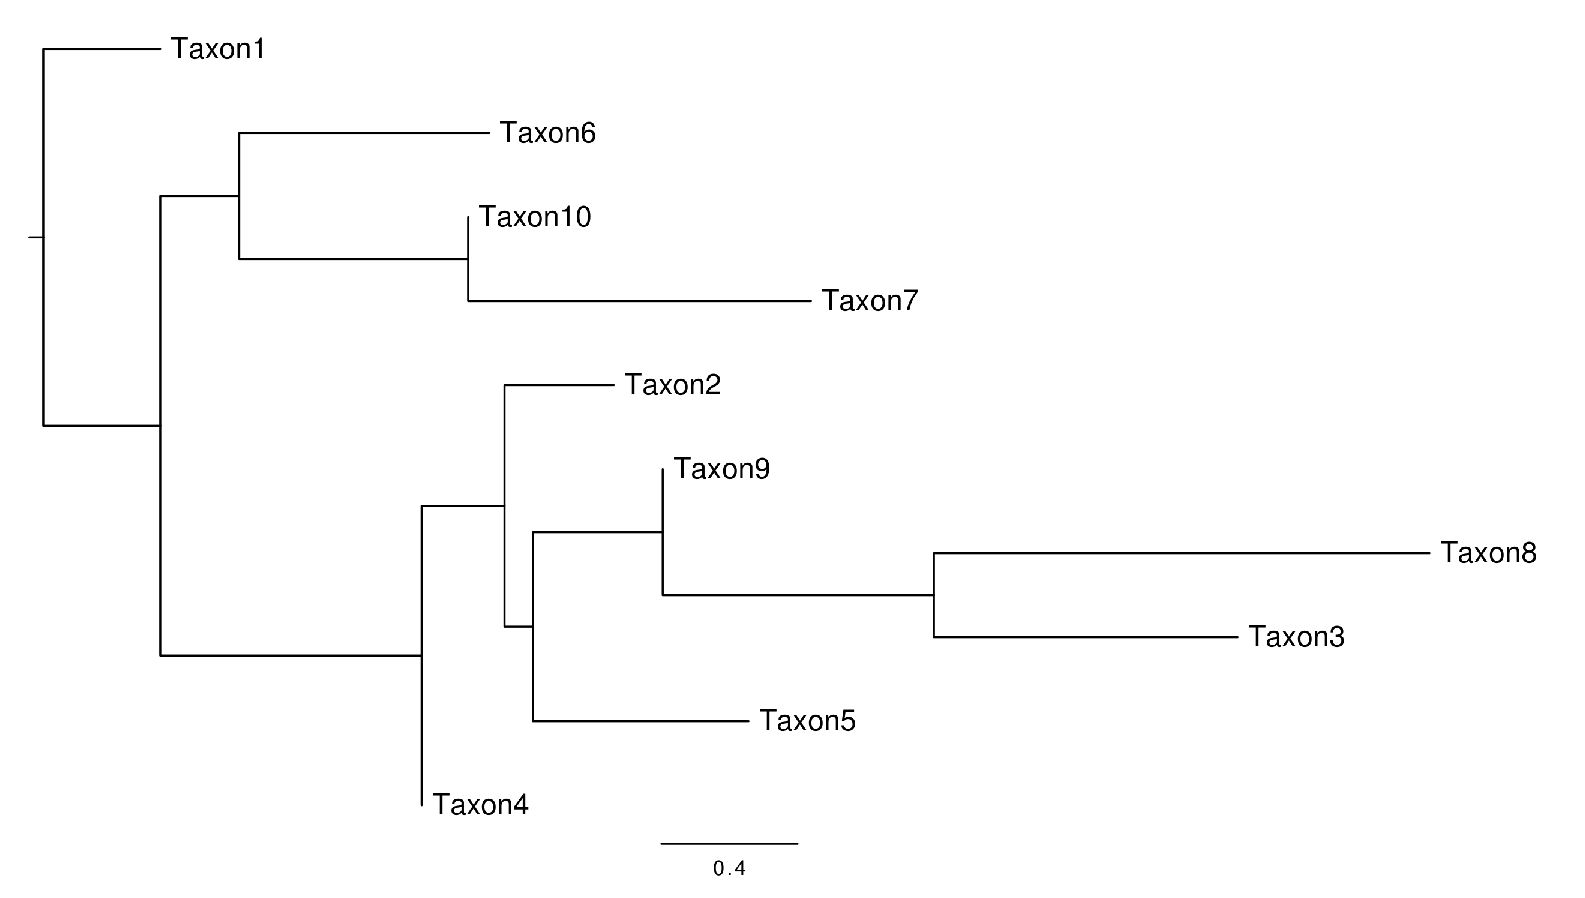
\includegraphics[scale=0.65]{figures/tut14/garlirunbest.eps}}
	{\caption[Topologia de verossimilhançca para \texttt{partition1+2aln3.nex}.]{Topologia selecionada sob o critério de Verossimilhança máxima dos dados em \texttt{partition1+2aln3.nex} com  $lnL$ -1369.5791.}\label{tut14:fig:treml}}

  \end{figure}

%%%%%%%%%%%%%%%%%%%%%%%%%%% FIM DA FIGURA MODELS IN POY %%%%%%%%%%%%%%%%%%%%%


\section{Suporte de Goodman-Bremer}\label{tut14:bremer}

Ao contrário dos valores de Bootstrap, o suporte de Goodman-Bremer ($GB$) \parencite{GoodmanETAL1982,Bremer1988} é uma medida empírica de suporte dado pela evidência a um determinado clado. Portanto, é considerado um valor de suporte direto. O suporte de Goodman-Bremer é a diferença de comprimento (\textit{i.e.}, custo, número de passos) entre o cladograma mais parcimonioso ($L$) e o cladograma mais parcimonioso que não apresenta um determinado clado de interesse ($L'$):

\begin{center}
\begin{equation}
GB=L'-L
\end{equation}
\end{center}

Em outras palavras, o valor de Goodman-Bremer representa o número adicional de passos em uma topologia sub-ótima necessário para colapsar determinado nó. Uma outra maneira de pensar sobre essa métrica é que o seu valor indica a quantidade relativa de contra-evidências necessária para que você não tenha suporte nenhum sobre determinado grupo. Vale considerar que o $GB$ é dependente do enraizamento da topologia e que grupos que estariam ausentes no consenso estrito, e portanto não são suportados pelas evidências, apresentam $GB=0$.\\

%%%%%%%%%%%%%%%%%%%%%%%%%%% FIGURA MODELS IN POY%%%%%%%%%%%%%%%%%%%%%%%%%%%
%  \vspace{-1em}
  \begin{figure}[h!]
    %\ffigbox[\FBwidth]
      {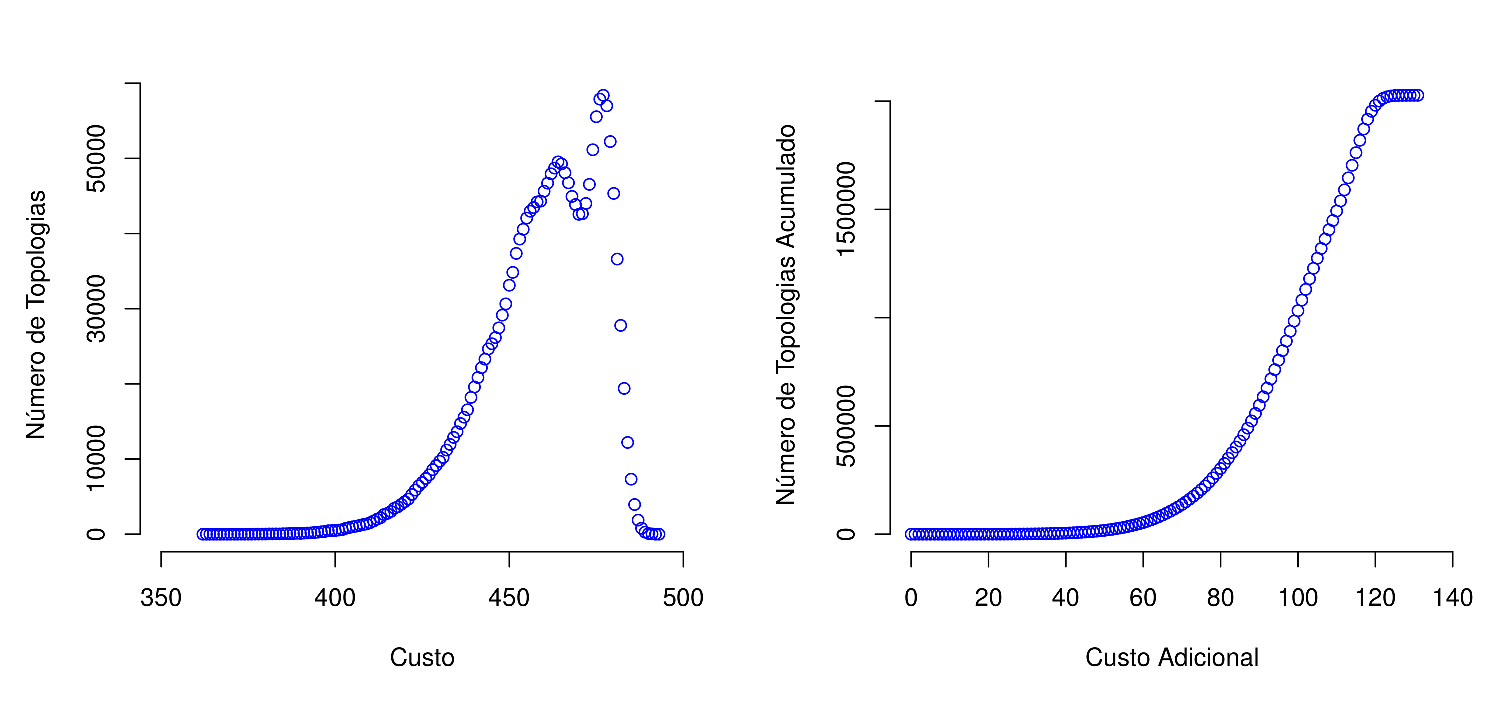
\includegraphics[scale=0.65]{figures/tut14/plot_alltrees.eps}}
	{\caption[Distribuição e acúmulo durante enumeração.]{Distribuição de topologias de acordo com seu custo (esquerda) e acúmulo de topologias de acordo com número de passos adicionais com relação à topologia mais curta para os dados do arquivo \texttt{total\_evidence.tnt} (direita).}\label{tut14:fig:bremer1}}
  \end{figure}

%%%%%%%%%%%%%%%%%%%%%%%%%%% FIM DA FIGURA MODELS IN POY %%%%%%%%%%%%%%%%%%%%%

Há algumas propriedades sobre esse índice que você deve considerar. Está claro que para computá-lo é necessário avaliar topologias sub-ótimas e isso pode ser um problema se você está diante de um espaço topológico complexo. Considere por exemplo o arquivo de dados \texttt{total\_evidence.tnt}. Neste arquivo estão concatenados os dados de \texttt{partition1.fas}, \texttt{partition2.fas} e \texttt{partition3.tnt}. A enumeração destes dados, que contém 10 terminais -- portanto 2.027.025 topologias possíveis, resulta em custos que variam de 362 a 493 (Figura \ref{tut14:fig:bremer1}). Suponha que para determinado nó, o índice de GB seja 120, você teria que ter avaliado praticamente todo o espaço de topologias. Felizmente, para esses dados, o clado com maior índice de GB é 14. Desta forma, para esses dados o cômputo desses índices parece ser trivial -- o que certamente não é o caso de muitos dados reais.

Há várias estratégias adotadas para calcular o índice de BG. Em sua forma mais primitiva, você poderia compilar todas as topologias com $n$ passos de distância da topologia mais curta que você obteve para seus dados e posteriormente, calcular passo a passo esse índice filtrando as topologias $c+n$, no qual $c$ é o custo mínimo e $n$ é o número de passos adicionais, calculando o consenso, e verificando quais nós são colapsados. Fazer isso manualmente é laborioso e demanda tempo computacional e analítico.

A melhor forma de calcular o índice de GB é utilizando um macro disponível em TNT chamado \texttt{BREMER.RUN}. Este macro utiliza buscas com os algoritmos de novas tecnologias para compilar de tologias sub-ótimas, que posteriormente são utilizadas para obter os índices. Para executar esse macro é necessário que você possua uma topologia na memória. Caso seus dados resultem um múltiplas topologias, o ideal seria você calcular o consenso estrito desta topologia, mantê-lo na memória e descartar as topologias fundamentais (veja Seção \ref{tut6:consenso} do Tutorial \ref{tut6}) e, finalmente, executar o macro do TNT.

O POY também permite o cálculo deste índice utlizando algumas de suas estratégias internas. Porém isso é feito assumindo homologia estática dos dados, uma vez que o uso de homologia dinâmica para esse propósito se mostrou computacionalmente inviável -- além de desnecessário. Sendo assim, considero mais efetivo submeter o alinhamento implícito das análises em POY para o cálculo de BG. Considere o exemplo abaixo:\\

\begin{lstlisting}[label=tut14:bs]
read("partition1.fas","partition2.fas","partition3.tnt")
set(root:"Taxon1")
search(max_time:0:0:5)
select()
set(iterative:exact)
swap(tbr)
fuse()
select(best:1)
transform (all, (static_approx))
report ("total_evidence.tnt", phastwinclad)
exit()
\end{lstlisting}

\vspace{35pt}

Neste \textit{script} (denominado \texttt{poy\_run.poy} e disponível no diretório deste tutorial), os dados são lidos e analisados utilizando os algoritmos de busca do comando \texttt{search} por 5 minutos, a melhor topologia e selecionada e rediagnosticada via \textit{Interative Pass} com refinamento, uma única topologia mais curta é selecionada, todos os dados são transformados em homologia estática e impresso no arquivo \texttt{total\_evidence.tnt} em formato TNT. Essa lógica analítica é uma boa estratégia para dados sujeitos a homologia dinâmica para os quais você deseja calcular índices que dependam de homologia estática -- e consequentemente valores de Bootstrap (caso você ainda considere esse último útil para alguma coisa). Para obter os valores de BG para esse arquivo, então, basta: (\textit{i}.) analisá-lo em TNT e obter uma topologia e (\textit{ii}.) executar o macro com o comando \texttt{run BREMER.RUN}.\\

\stepcounter{ex}
\begin{blackBlock}{\textbf{Exercicio 14.\arabic{ex}}}\label{tut14:ex:14.4}

Neste exercício você deverá obter os índices de bootstrap e GB para o arquivo \texttt{total\_evidence.tnt}. Use o espaço abaixo para desenhar a topologia e anotar os índices obtidos e, posteriormente, responda as seguintes perguntas:

\end{blackBlock}

\vspace{120pt}


\begin {myindentpar}{0.3cm}
\begin{enumerate}[\itshape i.]

	\item{Qual é o maior índice de GB que um determinado vértice (nó) pode possuir?}


\begin{center}
\line(1,0){400}\\
\line(1,0){400}\\
\line(1,0){400}\\
\end{center}


	\item{Existe alguma correlação entre os índices de bootstrap e GB?}

\begin{center}
\line(1,0){400}\\
\line(1,0){400}\\
\line(1,0){400}\\
\end{center}

\end{enumerate}
\end{myindentpar}

\section{Verossimilhança diferencial (\textit{Likelihood difference})}\label{tut14:lkr}

A Verossimilhança diferencial é equivalente ao índice de GB dentro do contexto de análises sob o critério de Verossimilhança. Embora pouco empregado \parencite[veja referências em][]{GrantKluge2008b}, esse índice possui todas as propriedades desejáveis de um índice de suporte \parencite[][]{Edwards_1992,GrantKluge2008b}. O índice é dado pela seguinte formulação:

\begin{center}
\begin{equation}
P(e|h,b) - P(e|h',b)
\end{equation}
\end{center}

no qual $h$ é a hipótese selecionada e $h'$ é a hipótese alternativa. Como GB, este índice está diretamente relacionado ao critério de otimalidade, e portando, deve ser considerado um índice de suporte direto. Dentro do contexto de análises filogenéticas, a diferença de Verossimilhança é aplicada em relação à topologia ótima e aquela considerada ótima na ausência do clado em questão Atualmente não há programas que possibilitam o cômputo imediato deste índice. Sua obtenção, portanto, dependerá de uma série de análises sequenciais que iremos demonstrar a seguir.

Suponha que seus dados estejam em \texttt{partition1+2aln3.nex} e que após selecionar o melhor modelo para sua análise, você configurou o arquivo \texttt{garli\_single.conf}, ambos disponíveis no diretório deste tutorial. O resultado desta análise (arquivos \texttt{garli\_run.*.*}) resultou em uma topologia com $lnL$ -1369.5791. Figura \ref{tut14:fig:treml} do Exercício 14.3 é resultado desta análise.

Para calcular a diferença de Verossimilhança para o clado (Taxon8+Taxon3) é necessário obter a topologia ótima na qual esse clado não existe. Isso é feito utilizando o que chamamos de buscas sob restrição reversa (\textit{reverse/negative constraint}). A primeira etapa seria definir a topologia que contém esse clado. Para esse caso em particular, seria:\\

\begin{center}
\scriptsize\texttt{(Taxon1,Taxon2,Taxon4,Taxon5,Taxon6,Taxon7,Taxon9,Taxon10,(Taxon8,Taxon3))}
\end{center}

Esta topologia deve estar contida em um arquivo texto com um sinal $-$ (negativo), que indica ao GARLI que ela deve ser utilizada como restrição reversa. Chamaremos esse arquivo de \texttt{contraint\_8+3.tre}. O próximo passo é editar o arquivo de configuração de GARLI. Para isso, uma cópia do arquivo \texttt{garli\_single.conf} foi feita e denominada \texttt{garli\_constrain.conf} e os comandos \texttt{ofprefix} e \texttt{constraintfile} foram modificados para o cálculo (veja conteúdo desses arquivos).

O resultado desta análise gerou uma topologia com $lnL$ -1369.8372, a qual é considerada a topologia ótima sob este critério na qual o clado (Taxon8+Taxon3) não existe. Para calcular a Verossimilhança diferencial para este clado, basta subtrair o $lnL$ da hipótese sob restrição reversa daquela obtida na primeira análise onde este clado foi recuperado. Assim

\begin{center}
\begin{equation}
LR_{T8+T3} = lnL_{com T8+T3} - lnL_{sem T8+T3}
\end{equation}
\end{center}

Portanto,


\begin{center}
\begin{equation}
LR_{T8+T3} = 0.2581.
\end{equation}
\end{center}

\vspace{50pt}

\stepcounter{ex}
\begin{blackBlock}{\textbf{Exercicio 14.\arabic{ex}}}\label{tut14:ex:14.5}

Neste exercício você deverá obter os índices das Razões de Verossimilhança para os cinco clados definidos abaixo, provenientes da Figura \ref{tut14:fig:treml}, utilizando as etapas descritas acima. Anote os valores obtidos na Figura \ref{tut14:fig:treml} e responda:

\end{blackBlock}

\vspace{50pt}

Clados de interesse:

\begin{center}

\scriptsize\texttt{(Taxon1,Taxon2,Taxon4,Taxon5,Taxon6,Taxon7,Taxon10,(Taxon9,Taxon8,Taxon3))}\\
\scriptsize\texttt{(Taxon1,Taxon2,Taxon4,Taxon6,Taxon7,Taxon10,(Taxon5,Taxon9,Taxon8,Taxon3))}\\
\scriptsize\texttt{(Taxon1,Taxon4,Taxon6,Taxon7,Taxon10,(Taxon2,Taxon5,Taxon9,Taxon8,Taxon3))}\\
\scriptsize\texttt{(Taxon1,Taxon6,Taxon7,Taxon10,(Taxon4,Taxon2,Taxon5,Taxon9,Taxon8,Taxon3))}\\

\end{center}


\begin {myindentpar}{0.3cm}
\begin{enumerate}[\itshape i.]

	\item{Existe alguma correlação observável entre os índices de Bootstrap obtidos no Exercício 14.3 e Verossimilhanca diferencial?}

\begin{center}
\line(1,0){400}\\
\line(1,0){400}\\
\line(1,0){400}\\
\end{center}

\end{enumerate}
\end{myindentpar}



%%%%%%%%%%%%%%%%%%%%%%%%%%%% HERE ENDS TEXT AND ADDS REFERENCES %%%%%%%%%%%%%%%%%%%%%%%%%%%% 
\newpage
\section{Referências}\label{tut14:refs}
\printbibliography[heading=none]
\end{refsection}
%
